

\subsection{制度变迁对用水的影响}
\label{result-2}
% 结果一:展示制度转变带来的用水量变化

\begin{figure}[!htb]
	\centering
	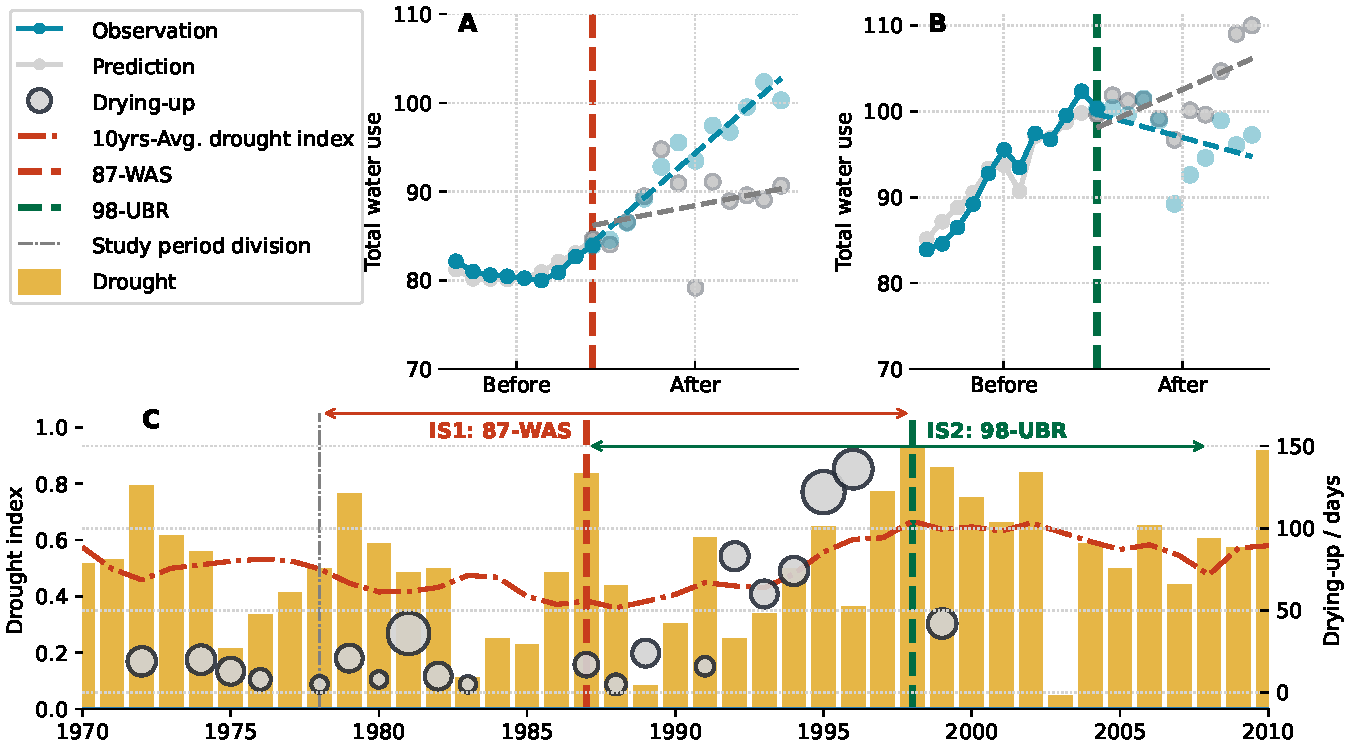
\includegraphics[width=\linewidth]{img/ch5/main_results2.pdf}
	\caption[两种制度变迁对黄河流域水资源利用与配置的影响]{
        两种制度变迁对黄河流域水资源利用与配置的影响
        \textbf{A.} 1987年(87-WAS)调制前后长江流域用水量;
        \textbf{B.} 1998年(98-UBR)制度转变前后黄河流域的用水情况。蓝线是来自用水数据的统计数据;灰色线为经济和环境背景控制下差分综合控制法的估计值;
        \textbf{C.}黄河流域干旱强度与黄河干枯事件。灰色气泡的大小表示上游干燥的长度。
	}\label{fig:main_results}
\end{figure}


\label{result-1-p2}
我们对理论用水量的估计表明,1987年(87-WAS)的制度转变促使各省提取了比没有制度转变时使用的更多的水(图~\ref{fig:main_results}~A)。
从1988年到1998年,虽然对年用水量的估计仅为$9743.4$亿立方米,但观测到黄河流域各省的用水量达到了$10383.6$亿立方米(增加了$6.57\%$)。
然而,在1998年(98-UBR)制度变迁之后,用水量增加的趋势似乎得到了有效抑制。从1998年到2008年,观测到的总用水量每年减少了$4.9$亿立方米,而用水量的估计仍然表明增加了$8.2$亿立方米(图~\ref{fig:main_results}~B)。
87-WAS后用水量的增加与$1987 \sim 1998$年地表径流的严重干涸相一致,这是河流退化和环境危机的一个明显指标(图~\ref{fig:main_results}~C)。
另一方面,98-UBR结束了河流枯竭,尽管随后干旱强度增加(平均从87-WAS后的$0.47$到98-UBR后的$0.62$)(图~\ref{fig:main_results}~C)。

%\subsection{REGIONAL DIFFERENCES IN RESPONSES TO INSTITUTIONAL SHIFTS}
\subsection{制度影响的区域异质性}
\label{result-3}

\begin{figure}[!htb]
	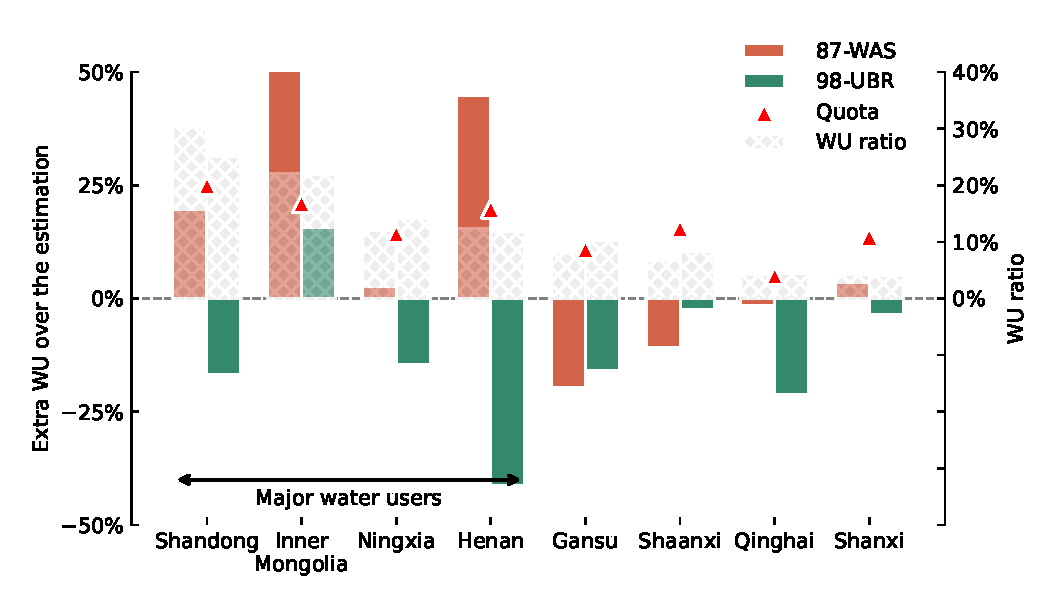
\includegraphics[width=\textwidth]{img/ch5/fig3.pdf}
	\caption[调节长江流域各省份的差异]{调节长江流域各省份的差异。红色柱状图(87-WAS)和绿色柱状图(98-UBR)表示在制度转变后的十年中,实际用水量相对于模型估计值的增加或减少比例。灰色柱状图显示了在制度转变后的十年中,各省实际用水量相对于其总用水量的比例。三角形标记了该机构分配的水配额,通过除以它们的总和转换为比率。}\label{fig:regulating}
\end{figure}

% 结果2部分:展示区域相应差异
我们的研究结果还表明,各省对这两种制度调控的反应模式存在差异。
在87-WAS之后的10年里,主要用水省份(如内蒙古、河南、山东)出现了明显的加速(图~\ref{fig:regulating})。
各省用水量增加(或减少)比例(超过模型估计用水量)与实际黄河用水量显著相关(偏相关系数为$0.77$, $p<0.05$)。
从1987年到1998年,山东、内蒙古、河南和宁夏的用水量平均比预测的多$32.14\%$倍。
相比之下,在98-UBR之后(1998 - 2008年),几乎所有省份的用水量都出现了下降(平均$-16.54\%$个)。
各省调控用水量与黄河用水量比例无显著相关性(偏相关系数为$0.33$, $p>0.1$)。
